% arara: xelatex
% arara: xelatex
% arara: xelatex

% options:
% thesis=B bachelor's thesis
% thesis=M master's thesis
% czech thesis in Czech language
% english thesis in English language
% hidelinks remove colour boxes around hyperlinks

\documentclass[thesis=B,czech]{FITthesis}[2012/10/20]

\usepackage[utf8]{inputenc}

\usepackage{graphicx} %graphics files inclusion

\usepackage{dirtree}

\usepackage{xevlna} %pouze u xelatexu

\usepackage{todonotes}

\usepackage{minted}

\newcommand{\tg}{\mathop{\mathrm{tg}}} %cesky tangens
\newcommand{\cotg}{\mathop{\mathrm{cotg}}} %cesky cotangens

% % % % % % % % % % % % % % % % % % % % % % % % % % % % % % 
% ODTUD DAL VSE ZMENTE
% % % % % % % % % % % % % % % % % % % % % % % % % % % % % % 

\department{Katedra softwarového inženýrství}
\title{Aplikace pro řízení a~správu vytápění v~chytré domácnosti s pomocí wifi sítě}
\authorGN{Lukáš} %(křestní) jméno (jména) autora
\authorFN{Hepner} %příjmení autora
\authorWithDegrees{Lukáš Hepner} %jméno autora včetně akademických titulů
\author{Lukáš Hepner} %jméno autora bez akademických titulů
\supervisor{Ing. Pavel Kubalík, Ph.D.}
\acknowledgements{Tímto chci poděkovat mému vedoucímu bakalářské práce, panu Ing.~Kubalíkovi,~Ph.D., za jeho výborné vedení, čas strávený na konzultacích a velmi přínosné rady. Dále bych rád poděkoval své rodině a kamarádům za jejich podporu během studia.}
\abstractCS{Práce se zabývá tvorbou aplikace pro řízení vytápění v chytré domácnosti. Aplikace umožňuje správu topných hlavic pomocí Wi-Fi sítě. Aplikace je určena pro operační systém Windows. Práce zkoumá existující řešení, obsahuje analýzu požadavků, implementaci a testování. Součástí práce je i návrh topné hlavice, se kterou aplikace komunikuje.

Aplikace je určena pro uživatele, kteří chtějí zefektivnit vytápění své domácnosti. Dává jim další možnost při výběru z omezeného množství výrobců. A nahrazuje speciální hardware pro správu topných hlavic.
}
\abstractEN{The thesis is dealing with creation of application, that controls heating in your smart home. The application allows you to manage and control heaters via Wi-Fi network. The application is designed for the Windows operating system. The thesis explores existing solutions, includes requirements analysis, implementation and testing. Part of the thesis is draft of the heater with witch the application communicates.

The application is designed for users who want to make their heating more efficient. It gives them another option when choosing from limited amount of manufactures. And replaces specialized hardware for managing the heaters.
}
\placeForDeclarationOfAuthenticity{V~Praze}
\declarationOfAuthenticityOption{4} %volba Prohlášení
\keywordsCS{chytrá domácnost, správa vytápění, Wi-Fi síť, Windows, .NET~Framework}%C# nebo .NET Framework
\keywordsEN{smart home, heating control, Wi-Fi~network, Windows, .NET Framework}
%\website{http://site.example/thesis} %volitelná URL práce, objeví se v tiráži


\begin{document}

\begin{introduction}
V dnešní době se chytré domácnosti začínají těšit značné popularitě. Díky nim lze domácnost snadno kontrolovat a nastavit automatické procesy, které ji budou řídit.

Práce se zaměřuje na automatické ovládání vytápění. To umožňuje nastavit komfortní teplotu pro spánek a tu opět automaticky zvýšit v době vstávání.
Kontrola vytápění taktéž napomáhá ke snížením nákladů. Například když člověk není doma nebo nevyužívá danou místnost.

V současné době však existuje malé množství systémů, které umožňují jednoduché nastavení. Existující řešení postrádají konkurenci a zákazník nemá možnost výběru.
Díky malé konkurenci se pořizovací cena systémů pro kontrolu vytápění pohybuje v řádu desítek tisíc korun. Což je pro spoustu lidí částka, kterou nejsou ochotni zaplatit.

Proto je cílem mé práce vytvořit další konkurenční řešení, které bude cenově přijatelnější a bude si ho moci dovolit více lidí. Tato práce zkoumá existující řešení a na jejich základě vytváří funkční požadavky. 

Další kapitola je věnována návrhu komunikace topné hlavice s~aplikací. Následuje implementační část, ve které jsou popsány vrstvy, ze kterých se aplikace skládá. V poslední části je aplikace podrobena testování.

%\todo{Představit strukturu práce... Teoretická, praktická část}


\end{introduction}

\chapter{Cíle}
Cílem práce je usnadnit uživateli ovládání vytápění v domácnosti, pomocí aplikace pro Windows. Aplikace bude umožňovat uživateli vytvářet rozvrhy vytápění pomocí grafického rozhraní a ty přiřazovat vybraným topným hlavicím. Topné hlavice bude možné přidávat a pojmenovávat.

Rozvrh vytápění bude možné uložit, následně jej přiřadit topným hlavicím a dle potřeby později upravit. Rozvrh je na týden a každý den může mít specifikované odlišné teploty. Topné hlavice a k nim přiřazené rozvrhy bude možné ukládat do profilů. Profily usnadňují změnu vytápěcího režimu v celé domácnosti -- všech topných hlavic -- najednou.

Další důležitou vlastností chytrých domácností je možnost nastavení temperace, pro zabránění promrzání. Aplikace umožní nastavení teploty, na kterou se má temperovat a datum návratu, kdy se má začít vytápět podle normálního rozvrhu.

Aplikace bude umožňovat správu uživatelských účtů s různými oprávněními. Někteří uživatelé budou mít pouze právo na zobrazení aktuální teploty. Jiní i pro vytváření a úpravu rozvrhů vytápění.

Práce se také zabývá návrhem a implementací topné hlavice, se kterou bude aplikace komunikovat.

\chapter{Rešerše}

\section{Existující řešení}

Při vytváření nového produktu je nutné prozkoumat současný stav trhu a~zjistit, zdali pro něj existuje místo a potenciální zákazníci. Konkurenční produkty byly vybírány tak, aby umožnily vylepšení topné soustavy bez nutnosti stavebních úprav. U těchto produktů byly následně zkoumány jejich přednosti, výhody a~nevýhody.

\subsection{Tado° }
Tado° poskytuje nástroje pro ovládaní vytápění a chlazení domu. Tado° dodává vlastní hlavice na radiátory, které komunikují s centrálním termostatem a udržují teplotu v místnosti. Termostat má tři tlačítka pro nastavení teploty a rozvrhu vytápění. Toto nastavení je však poměrně komplikované, neboť ovládání je limitováno třemi tlačítky.

Proto Tado° dodává mobilní aplikaci, která s termostatem komunikuje a~zjednodušuje nastavení. Mobilní aplikace ukazuje aktuální teplotu v jednotlivých pokojích a umožňuje její editaci ve vytápěcím rozvrhu. Aplikace sleduje polohu členů domácnosti a podle ní upravuje rozvrh vytápění. Nevýhodou však je, že všichni členové domácnosti musí mít chytrý telefon s nainstalovanou aplikací a~ten nosit neustále při sobě. Aplikace sleduje předpověď počasí a podle ní upravuje rozvrh vytápění. 

Aplikace však postráda přehledný graf, kde by uživatel viděl, na jakou hodnotu je teplota nastavena v průběhu dne.
Termostat má senzor vlhkosti a~dokáže uživatele upozornit, aby vyvětral a předešel tak tvorbě plísně. Hlavice a termostat dokáží rozpoznat otevřené okno a přestat vytápět, což snižuje náklady na vytápění.

Hlavice s termostatem spolu komunikují na frekvenci 868 MHz. Komunikace s aplikací probíhá přes most, připojený k routeru, který komunikuje s~termostatem.

Systém Tado° lze připojit do chytré domácnosti pomocí Apple HomeKit. Termostat je možné ovládat pomocí Siri, Google Assistant nebo Amazon Alexa.

Tado° nabízí termostat na zeď: Smart Thermostat -- Starter Kit V3+, který se prodává za 199,99 €. A chytrou hlavici na radiátor: Smart Radiator Thermostat -- Starter Kit V3+, za 129,99 €. Tato částka představuje nemalou investici, pokud chceme všechny radiátory vybavit chytrými hlavicemi~\cite{tado}.

\subsection{Honeywell}

Honeywell poskytuje řadu termostatů, které ovládají teplotu centrálně a neumožňují nastavení teploty v jednotlivých místnostech. Termostaty mají dotykové obrazovky pro snazší ovládání a umožnují nastavení rozvrhu vytápění na sedm dní.

Termostat lze připojit k Wi-Fi a ovládat ho pomocí aplikace v mobilním telefonu nebo počítači. Zde taky můžete dostávat upozornění na špatné počasí.

Termostat umožňuje dělat rychlé změny v rozvrhu, dočasné změny teploty nebo režim dovolené. Lze zde nastavit heslo pro přístup pouze oprávněných osob.
Také zde chybí graf vývoje teploty.

Termostat lze ovládat pomocí Amazon Alexa, SmartThings a Google Assistant. Nenabízí podporu Apple HomeKit nebo ovládání pomocí Siri.

Termostat od Honeywellu RTH9585WF1004 Wi-Fi, se prodává za \$199,99. Honewell dále nabízí řadu hlavic, které se pohybují v cenové relaci \$60--\$80. Například: Honeywell HR92EE, která stojí \$60 ~\cite{honey}.

\subsection{Závěr}

Současných řešení na trhu není mnoho a zákazník si často nemůže vybrat z~více produktů vyhovujících jeho požadavkům. Trh s chytrými domácnostmi se teprve začíná rozvíjet a spousta výrobců stále spoléhá pouze na dedikovaný hardware pro ovládání teploty. Termostaty se často složitě ovládají a~nastavení teploty je zdlouhavé. Některé typy termostatů se po restartu vymažou a~uživatel je nucen opakovaně zadávat data, a proto často přestane tuto funkcionalitu využívat.

Je nutné vytvořit aplikaci umožňující rychlou a snadnou změnu nastavení. Pro běh aplikace je ideální počítač, protože uživatel může používat myš a~klávesnici (popřípadě dotykovou obrazovku) namísto několika tlačítek na termostatu. Zároveň by měl mít možnost předdefinovat si různé profily vytápění a mezi nimi jednoduše přepínat.

Díky nedostatečné konkurenci si firmy mohou diktovat ceny a zákazník je nucen zaplatit desítky tisíc za vybavení domácnosti.

\chapter{Analýza}

\section{Volba technologií}

Pro tvorbu aplikace na ovládaní termostatických hlavic, jsem si zvolil programovací jazyk C\#. Aplikace bude spustitelná na systému Windows. Ten byl vybrán pro jeho rozšířenost v domácnostech viz. tabulka \ref{table:2}. Aplikace pro PC se snadno ovládají díky myši a klávesnici. Jednoduchost použití je velice důležitá, jinak ji uživatel přestane používat. Aplikace půjde zároveň spouštět i~z~tabletů s~operačním systémem Windows, který může sloužit jako ovládací jednotka pro chytrou domácnost.

     \begin{table}[]
         \begin{tabular}{lc}
            Operační systém & Procentuální zastoupení \\
            \hline
           Windows         & 79,46                   \\
           OS X            & 14,35                   \\
           Linux           & 1,7                     \\
           Ostatní         & 4,49                   
       \end{tabular}
\caption{Zastoupení operačních systémů na trhu~\cite{osPer}}
\label{table:2}
\end{table}

Jako vývojová deska pro prototyp hlavice byl zvolen WeMos D1~\cite{wemos}, která má v sobě zabudovaný Wi-Fi modul ESP8266, který dokáže komunikovat na frekvenci 2,4~GHz. Routery pracující na frekvenci 2,4~GHz jsou velmi rozšířené a mají lepší prostupnost signálu než routery pracující na frekvenci 5~GHz. Desku lze využít jako Arduino čip, pro který existuje celá řada knihoven a~usnadní tak vývoj. WeMos D1 obsahuje řadu pinů, které jsou užitečné pro snadný vývoj. V hotovém řešení může být použita menší deska se stejným mikročipem -- ESP8266.

Data aplikace se budou serializovat do formátu XML. Tento formát je snadno čitelný a lze využít namespace System.Xml.Linq~\cite{linq}, který umožňuje snadnou manipulaci s XML v paměti.
\newline
\newline
\indent Aplikace komunikuje s hlavicemi přes TCP protokol. Ten zajišťuje spolehlivé doručení ve správném pořadí~\cite{tcp}.

\section{Funkční požadavky}

\subsection{Rozvrh vytápění}

Uživatel bude moci nastavit teplotu pro jednotlivé místnosti na 7 dní v týdnu. Po 10 minutách s přesností 0,1 °C. Rozvrh bude uložen na EEPROM desky, kvůli zachování nastavení při restartu. Teplotu bude možné nastavit v rozsahu 10–30 °C, tudíž bude moci být uložena v jednom bytu, $(30 - 10) \cdot 10 + 1 = 201 <= 255$. Rozvrh bude zabírat $7 \cdot 24 \cdot 6 \cdot 1 = 1008B$.

\subsection{Přihlášení do aplikace}

Pro změnu rozvrhu bude muset být uživatel přihlášen ke stejné Wi-Fi jako ostatní hlavice, tím se zamezí přístup neoprávněným uživatelům (neznajícím heslo k Wi-Fi). Při prvním spuštění se bude uživatel muset přihlásit pod administrátorským účtem, u kterého bude muset změnit heslo.

\subsection{Přidání uživatelů}

Administrátor bude moci vytvářet uživatelské účty, které budou mít pouze právo pro čtení dat z aplikace. Pro editaci údajů se bude muset uživatel přihlásit k administrátorskému účtu.

\subsection{Přidání hlavic}

Uživatel bude moct postupně přidávat hlavice a ty si v aplikaci pojmenovat. Nové hlavice budou identifikovány pomocí počátečního ID. Každá pojmenovaná hlavice si do EEPROM zapíše kód o velikosti dva byty, podle kterého se bude aplikaci identifikovat. 

Uživatel bude muset přidat vždy pouze jednu hlavici a tu pojmenovat, aby v síti nebylo více hlavic s~duplicitním ID.


\subsection{Vytvoření rozvrhu vytápění}

Uživatel bude moci vytvořit vytápěcí rozvrh na týden. To buď v grafu nebo nastavením jednotlivých časů, kdy má dojít ke změně na požadovanou hodnotu.

Při vytváření si uživatel bude moci vybrat, ke kterým dnům nastaví vytvořenou křivku teplot. Rozvrh vytápění si poté pojmenuje a uloží.


\subsection{Editace rozvrhu vytápění}

Při vytváření rozvrhu si uživatel bude moci vybrat již existují rozvrh a~k~němu přiřadit nové hodnoty. Změněné dny se poté uloží a přepíší původní rozvrh. Hodnoty, které uživatel nezmění, zůstanou stejné.

\subsection{Zobrazení rozvrhu vytápění}
Uživatel může zobrazit nastavení rozvrhu vytápění. Při jeho zobrazení se načtou všechny dny a zobrazí se v grafu teplot.

\subsection{Vybrání aktivního profilu}

Aplikace zobrazí vytvořené profily, uživatel jeden profil vybere a nastaví ho jako aktuální (profil podle kterého se má vytápět).

\subsection{Vytvoření vytápěcího profilu}

Uživatel může vytvořit vytápěcí profil, v němž je uložen seznam hlavic. Každá hlavice má přiřazený rozvrh vytápění. Poté, co uživatel každé hlavici přiřadí rozvrh vytápění, může si tento profil pojmenovat a uložit.

\subsection{Editace vytápěcího profilu}

Uživatel vybere vytápěcí profil, který si přeje editovat. Zobrazí se mu seznam aktuálních hlavic a jejich rozvrhů vytápění. Tento seznam může měnit, stejně tak může změnit název profilu.

\subsection{Režim dovolené}

Uživatel bude moct nastavit režim dovolená, kde zvolí požadovanou teplotu v~rozsahu 4--20 °C s přesností na celé stupně. Dále nastaví datum návratu, kdy má hlavice začít vytápět místnost na teplotu nastavenou v rozvrhu. Uživatel bude moci zrušit režim dovolené – začne se vytápět podle nastaveného rozvrhu.

Příkaz pro změnu rozvrhu se pošle všem připojeným hlavicím, aby uživatel nemusel manuálně nastavovat každou hlavici.

Pokud uživatel nechce všem hlavicím nastavit stejnou teplotu, může si vybrat profil, podle kterého se bude do jeho návratu vytápět.

\section{Nefunkční požadavky}

\subsection{Platforma Windows}

Aplikace půjde spustit na platformě Windows s verzí .NET Framework 4.7.2 nebo vyšší. .NET Framework podporuje volbu hashovací funkce, pro uložení a načítání hesla, až od verze 4.7.2.

\section{.NET Framework}

Aplikace je cílená na verzi .NET Framework 4.7.2, tato verze přidává nové konstruktory třídě Rfc2898DeriveBytes, která je využívána k~ukládání hesel. Tyto konstruktory umožňují specifikovat jméno algoritmu použitého pro hashování. Původní verze používá algoritmus SHA1, který se v dnešní době již nedoporučuje používat~\cite{netNews}.

Verzi 4.7.2 je možné nainstalovat na zařízení používající operační systém Windows 10, Windows 8.1 a~Windows 7 SP1~\cite{netNews}. Díky tomu půjde aplikace spustit na 95,45~\% (viz tabulka~\ref{table:1}) ze všech zařízení se~systémem Windows. 

\begin{table}[]
\begin{tabular}{lc}
Operační systém & Procentuální zastoupení \\
\hline
Windows 10      & 55,77                   \\
Windows 7       & 33,41                   \\
Windows 8.1     & 6,27                    \\
Windows XP      & 1,74                    \\
Windows 8       & 2,20                    \\
Windows Vista   & 0,55                    \\
Ostatní         & 0,06                   
\end{tabular}
\caption{Zastoupení operačních systémů Windows na trhu~\cite{windowsPer}}
\label{table:1}
\end{table}

\chapter{Návrh}

\section{Architektura}

Aplikace se skládá ze tří vrstev. To jí umožnuje rozdělit na tři logické celky.

\begin{description}
	\item[Prezentační vrstva] Využívá Windows Forms Application.
	\item[Aplikační vrstva] Je napsaná v C\# a poskytuje rozhraní, které může volat prezentační vrstva.
	\item[Datová vrstva] K ukládání dat využívá soubory ve formátu XML. Poskytuje rozhraní pro aplikační vrstvu. 
\end{description}

Díky tomuto rozdělení lze snadno vyměnit jednu vrstvu za druhou, pouze při zachování definovaných rozhraní. Rozdělení je velmi výhodné, protože lze snadno vyměnit prezentační nebo datovou vrstvu za jinou. Toto je důležité, pokud aplikace chce poskytovat i jiné uživatelské rozhraní například pro web nebo mobilní zařízení.

\begin{figure}\centering
	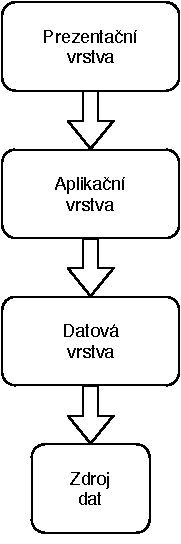
\includegraphics{diagrams/Architektura}
	\caption[Architektura aplikace]{Architektura aplikace}\label{fig:architektura}
\end{figure}

Z obrázku \ref{fig:architektura} je vidět, že každá vrstva dává požadavky pouze vrstvě pod sebou. Nikdy ne vrstvě nad sebou. Tímto se sníží provázání aplikace a je umožněno rozdělení do vrstev, které na sobě nejsou vzájemně závislé.

\section{Komunikace}

Aplikace bude komunikovat s hlavicí přes Wi-Fi pomocí TCP protokolu. TCP zajistí doručení dat ve správném pořadí. A na rozdíl od UDP zajistí spolehlivé doručení ~\cite{tcp}. Za spolehlivé doručení je považováno využívání kontrolního součtu paketu. 

TCP zajišťuje spolehlivé doručení na transportní vrstvě. Ale i přesto zde může nastat chyba. K této chybě však dochází jen s malou pravděpodobností. Pokud by docházelo k velkému počtu chyb, musela by se kontrola provádět nejen na transportní vrstvě, ale i na aplikační, a to například posláním hashe dat a následné kontroly, jestli se hashe rovnají.

\subsection{Topná hlavice}

Každá topná hlavice představuje server, ke kterému se připojuje klient (aplikace). Systém je takto navržen, protože hlavice jsou neustále v provozu a~tak se hodí pro funkci serveru. Dalším důvodem pro tuto konfiguraci je fakt, že komunikaci vždy započne klient (aplikace), topné hlavice nikdy neposílají aplikaci žádná data, která by si aplikace nevyžádala.

Systém může být tvořen více topnými hlavicemi, aplikace proto představuje skupinu klientů, kde je každý připojen právě k jedné topné hlavici. Tuto situaci zobrazuje obrázek~\ref{fig:comAppHeat}. Komunikace tak může probíhat paralelně. 

\begin{figure}\centering
	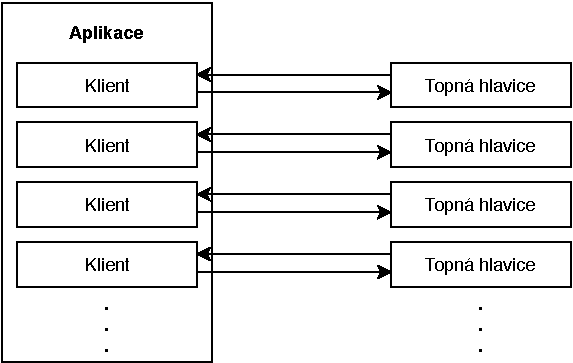
\includegraphics{diagrams/KomunikaceAppHeaters}
	\caption{Komunikace mezi aplikací a topnými hlavicemi}\label{fig:comAppHeat}
\end{figure}

\section{Uživatelé}
Uživatelé se dělí na dva typy podle jejich oprávnění – administrátor a ostatní uživatelé. Administrátor může vytvářet rozvrhy a profily vytápění, ty upravovat a přiřazovat vybraným hlavicím. Hlavice pojmenovávat, zobrazovat teplotu, vytvářet nové uživatele a využívat funkci dovolená. Ostatní uživatelé mohou pouze zobrazovat aktuální teplotu na topných hlavicích. Tyto akce zobrazuje obrázek~\ref{fig:uzivatele}.

\begin{figure}\centering
	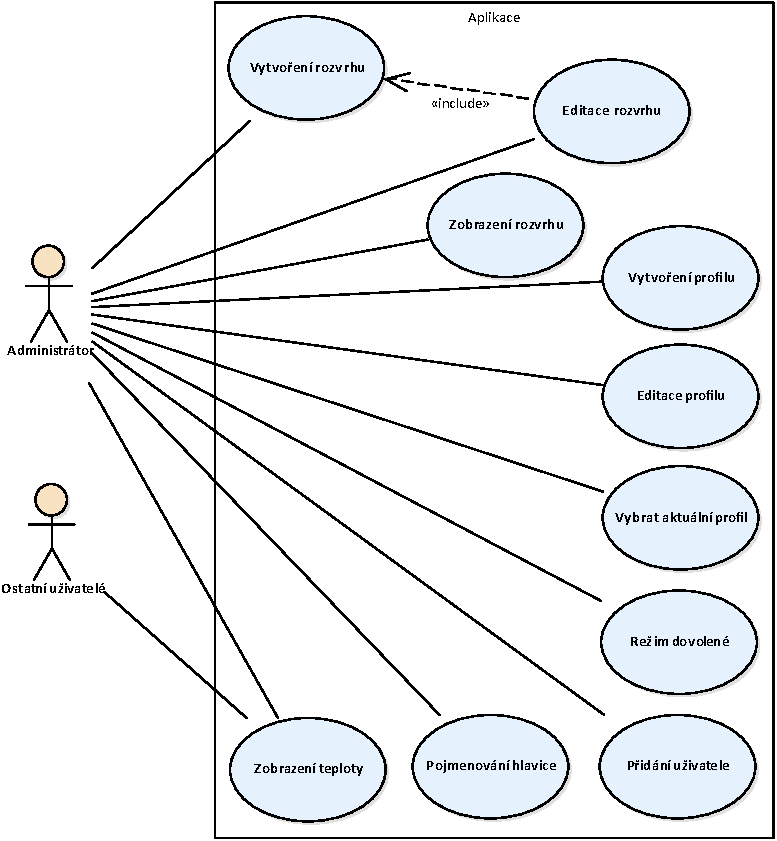
\includegraphics[width=\textwidth]{diagrams/Uzivatele}
	\caption[Uživatelské akce]{Diagram užití -- Uživatelské akce}\label{fig:uzivatele}
\end{figure}

\subsection{Vytvoření rozvrhu}

Administrátor může v aplikaci vytvořit rozvrh, a to buď v grafu teplot, nebo nastavením požadované teploty a času pomocí číselníků. Při vytváření rozvrhu si může vybrat pro jaké dny v týdnu bude platný. Poté rozvrh pojmenuje a~uloží.

\subsection{Editace rozvrhu}

Akci upravení rozvrhu předchází akce vytvoření rozvrhu. Při uložení rozvrhu administrátor zvolí jméno již existujícího rozvrhu, ve kterém jsou následně upraveny dny definované novým rozvrhem.

\subsection{Zobrazení rozvrhu}

Administrátor může zobrazovat existující rozvrhy vytápění.

\subsection{Vytvoření profilu}

Administrátor může vytvářet vytápěcí profily. Při vytvoření profilu se zobrazí seznam topných hlavic, ke kterým musí vybrat požadované rozvrhy vytápění. Poté profil pojmenuje a uloží.

\subsection{Editace profilu}

Administrátor vybere již existující profil, u kterého změní rozvrhy vytápění u vybraných hlavic. Pokud nechce měnit rozvrhy vytápění, může profil pouze přejmenovat a~uložit.

\subsection{Vybrat aktuální profil}

Pro změnu vytápěcího profilu, administrátor vybere požadovaný profil z nabídky a zvolí ho za aktuální. Rozvrhy uložené v profilu se rozešlou patřičným topným hlavicím a ty podle nich začnou vytápět, toto neplatí, pokud je nastaven režim dovolené. V tomto případě se topným hlavicím změní vytápěcí rozvrh, podle kterého se má vytápět po skončení režimu dovolené.

\subsection{Režim dovolené}

Administrátor může nastavit režim dovolené, kde si nastaví datum návratu a~požadovanou teplotu nebo profil, podle kterého se bude vytápět. Aplikace zajistí, aby se požadavek na zapnutí režimu dovolené rozeslal na všechny topné hlavice. Pokud chce administrátor zrušit režim dovolené například kvůli dřívějšímu návratu, stačí zvolit dřívější návrat. Aplikace opět rozešle požadavek všem hlavicím a ty začnou vytápět podle nastaveného rozvrhu.

\subsection{Přidání uživatele}

Administrátor má možnost vytvářet další uživatelské účty, které mají právo pouze pro čtení dat z aplikace. Administrátor zvolí uživatelské jméno, které ještě neexistuje, a heslo k účtu.

\subsection{Pojmenování hlavice}

Administrátor může zobrazit seznam topných hlavic, které může pojmenovat nebo jim změnit jméno. Pro uložení musí být každá hlavice pojmenovaná.

\subsection{Zobrazení teploty}

Každý uživatel může zobrazit seznam topných hlavic aktuálně připojených k~síti Wi-Fi, u kterých se mu zobrazí aktuální teplota.

\section{Komunikace hlavic s aplikací}

Aplikace komunikuje s topnými hlavicemi pomocí akcí, které jsou popsány na obrázku \ref{fig:komunikace}.

\begin{figure}\centering
	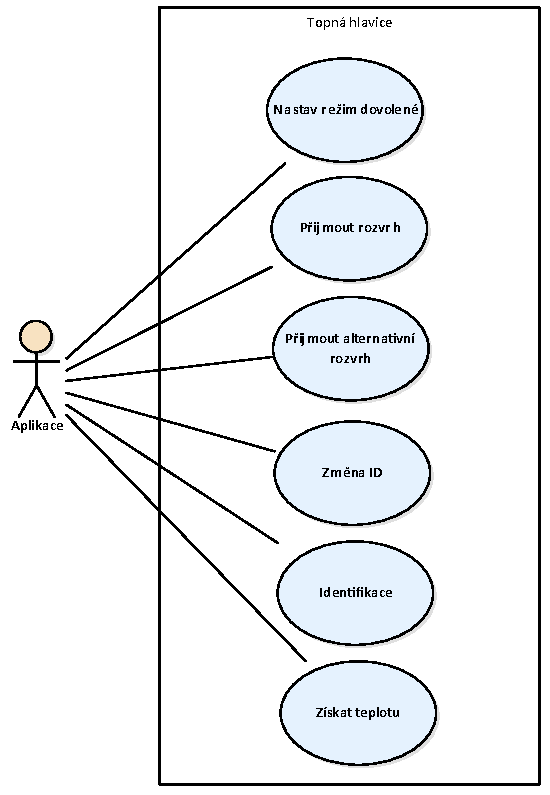
\includegraphics{diagrams/UCKomunikace}
	\caption[Komunikace aplikace s hlavicí]{Diagram užití -- Komunikace aplikace s hlavicí}\label{fig:komunikace}
\end{figure}

\subsection{Přijmout rozvrh}

Aplikace vytvoří požadavek na změnu rozvrhu, obsahující seznam dvojic -- časový údaj a požadovaná teplota. Posílá se vždy nový rozvrh vytápění -- topná hlavice starý rozvrh přepíše novým.

\subsection{Přijmout alternativní rozvrh}

Akce probíhá stejně jako u přijmutí rozvrhu, ale topná hlavice si rozvrh uloží na jiné místo v paměti.

\subsection{Nastav režim dovolené}

Aplikace vytvoří požadavek na nastavení režimu dovolené, kdy hlavice udržuje stálou teplotu. Požadavek obsahuje datum návratu a zvolenou teplotu (z~rozsahu 4--20~°C), na kterou se má domácnost vytápět. Topná hlavice kontroluje, zdali je nastaven datum návratu, který je alespoň o den větší než aktuální. 

Pokud uživatel nastavil profil vytápění, který má být zapnutý v režimu dovolené, vytvoří se požadavek s teplotou 0~°C. Teplota není validní a topná hlavice proto začne vytápět podle alternativního rozvrhu.

Pro zrušení režimu dovolené tedy stačí vytvořit požadavek s aktuálním datem, podmínka nebude splněna a hlavice začne vytápět podle nastaveného rozvrhu vytápění.


\subsection{Změna ID}

Všechny topné hlavice mají při prvním spuštění nastaveno počáteční ID, které je označuje za nové. Pro jejich identifikaci vygeneruje aplikace nové ID, odešle ho topné hlavici a ta si ho uloží do paměti EEPROM, aby ji bylo možné identifikovat i po restartu.

\subsection{Identifikace}

Topná hlavice se musí umět aplikaci identifikovat, aby mohla být spojena s~daty v aplikaci. Aplikace odešle požadavek na identifikaci topné hlavici a~čeká na odpověď. Topná hlavice načte ID z EEPROM a odešle ho aplikaci.

\subsection{Získej teplotu}

Aplikace odešle topné hlavici požadavek na sdělení teploty. Topná hlavice změří aktuální teplotu, kterou ořízne na dvě desetinná místa a odešle ji zpět aplikaci.

\chapter{Realizace aplikace}

\section{Použití tří vrstvé architektury}

%\verb|int main()|

% pracuji s tim jako s obrazkem 
% \begin{figure}
%\begin{verbatim} kod jako cerny text
%\end{verbatim}
% \end{figure}

%\mintinline{c++}|int main()|
Aplikační vrstva poskytuje rozhraní \mintinline{csharp}|IController|, které implementuje třída \mintinline{csharp}|Controller|.

\begin{minted}{csharp}
public interface IController
{
    Users.Response Login(String name, String pass);
    bool CreateUser(String name, String pass);
    bool IsUserAdmin();

    void SaveSchedule(Schedule schedule);
    List<Schedule> GetSchedules();

    List<Profile> GetProfiles();

    Heaters FindHeaters();
    void SaveHeatersAndActiveProfile(List<Heater> heaters,
                                     string profileName);
    void SaveNewHeatersAndNonactiveProfile(List<Heater> heaters,
                                     string profileName);

    void SetReturnDateAndTemperature(DateTime date, int temp);
    void SetReturnDateAndProfile(DateTime date, Profile profile);
    void EarlyReturn();
    Dictionary<String, double> GetTemperature();
}
\end{minted}

Tyto metody pak volá třída \mintinline{csharp}|Presenter|.

Controller volá metody rozhraní \mintinline{csharp}|IData|, které implementuje třída \mintinline{csharp}|Data|. 

\newpage

\begin{minted}{csharp}
public interface IData
{
    void SaveUsers(List<User> users);
    List<User> LoadUsers();

    void SaveSchedules(List<Schedule> schedules);
    List<Schedule> LoadSchedules();

    void SaveProfiles(List<Profile> profiles);
    List<Profile> LoadProfiles();

    void SaveHeaters(Heaters heaters);
    Heaters LoadHeaters();
}
\end{minted}

Třída \mintinline{csharp}|Data| ukládá informace pomocí LINQ do souboru.

Každá vrstva tak zná pouze rozhraní vrstvy se kterou komunikuje a nestará se o její implementaci.

\section{Prezenční vrstva}

Prezenční vrstva používá technologii Windows Forms, která umožňuje tvorbu formulářových aplikací. Uživatelské rozhraní je ovládáno třídou \mintinline{csharp}|Presenter|, která zajišťuje zpracování uživatelem prováděných akcí a komunikuje s aplikační vrstvou, ze které získává potřebná data. Třída \mintinline{csharp}|Presenter| zároveň zajišťuje, aby uživatelé, kteří nemají administrátorská práva nemohli měnit data aplikace, ale pouze si mohli zobrazit aktuální teplotu na topných hlavicích.

\subsection{Windows Forms}

\textit{
Windows Forms je klientská technologie pro .NET Framework, sada spravovaných knihoven, které zjednodušují běžné úkony jako je čtení a zápis souborů
} \cite{winForms}. Dále umožňuje vytváření událostí, které vyvolá uživatel, např. kliknutím myši nebo stiskem klávesy.

Knihovny dále poskytují řadu ovládacích prvků, jako jsou tlačítka, textová pole nebo číselné vstupy. Ty umožňují od uživatele získávat informace, zpracovat je a zobrazit mu výsledek operace.

\subsection{Graf vývoje teploty v čase}

Součástí .NET Frameworku jsou i knihovny pro práci s grafikou, které poskytují nástroje pro kreslení od základních tvarů až po vytváření obrazců pomocí Bézierových křivek~\cite{bezier}.

Tohoto je využito ve třídě \mintinline{csharp}|TemperatureGraph|, která vytvoří kreslící plochu s časovou a teplotní osou viz. obrázek \ref{fig:graf}. Zde je červenou barvou vykreslen ideální průběh teplot, tohoto průběhu však v praxi nelze dosáhnout. Proto se vykreslí další křivka – zelenou barvou – ukazující průběh teplot, blížící se reálnému chování.\footnote{Přesný vývoj teplot samozřejmě nelze odhadnout a bude se lišit místnost od místnosti. Hodnoty jsou proto určeny experimentálně na základě pozorování.} Křivky jsou vykreslené pomocí funkce  \mintinline{csharp}|DrawBezier|, určené pomocí počátečního, koncového a dvou kontrolních bodů. 

Uživatel klikáním na místa v grafu nebo výběrem z číselníku může nastavit požadované hodnoty. Po zadání hodnoty se graf překreslí podle nových hodnot.

\begin{figure}\centering
	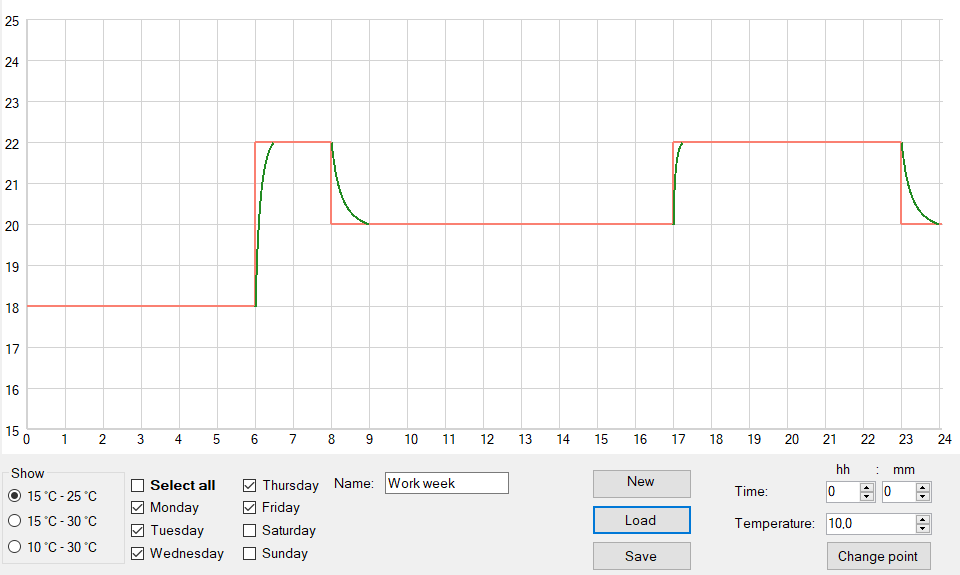
\includegraphics[width=\textwidth]{diagrams/Graf}
	\caption[Graf vývoje teploty]{Graf vývoje teploty}\label{fig:graf}
\end{figure}

\subsubsection{Změna hodnot}

Uživatel může opětovným kliknutím hodnotu odstranit. Aby byl výběr hodnoty zjednodušen, prozkoumává se blízké okolí bodu, kam uživatel klikl a zde se hledá již existující bod. Velikost prohledávaného okolí se odvíjí od šířky kreslící plochy -- počtu hodin, které graf zobrazuje (v aplikaci graf zobrazuje 24~hodin).

Pokud uživatel zadá teplotu v čase, kterému již teplota byla přiřazena, původní hodnota se nahradí novou. Aby bylo vždy jednoznačně možné určit, na kterou teplotu se má, v který čas vytápět.

\subsection{Zobrazení rozvrhu vytápění}

Pro zobrazení rozvrhu vytápění se využívá třídy  \mintinline{csharp}|TemperaturegraphSimple|, dědící z třídy  \mintinline{csharp}|TemperatureGraph|. Dědičnost je využita z~důvodu minimální odlišnosti tříd. Třída  \mintinline{csharp}|TemperaturegraphSimple| používá jiné vykreslování gra\-fu, ten zobrazuje pouze červenou křivku, nezobrazuje reálný průběh teploty a~popisky os viz. obrázek \ref{fig:grafVyber}. Ostatní chování zůstává nezměněné.

Při zobrazení rozvrhu vytápění, se pro každý den vytvoří nová instance třídy  \mintinline{csharp}|TemperaturegraphSimple|, ty jsou poté vykresleny v novém okně s popisky dnů. Pokud bylo okno zobrazeno na základě požadavku pro načtení rozvrhu vytápění k jeho editaci, je uživatel vyzván aby klikl na jeden z grafů a ten se poté načte do hlavního okna aplikace, kde ho je možné editovat.
\newline

\begin{figure}\centering
	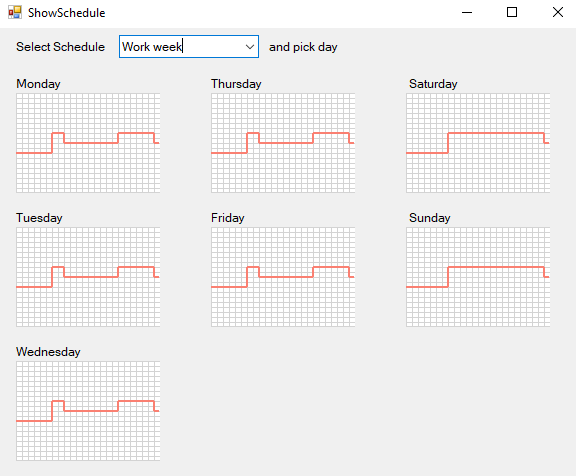
\includegraphics[width=\textwidth]{diagrams/GrafVyber}
	\caption{Zobrazení rozvrhu vytápění}\label{fig:grafVyber}
\end{figure}

\section{Aplikační vrstva}

Aplikační vrstva zprostředkuje komunikaci mezi prezenční vrstvou, datovou vrstvou a topnými hlavicemi. Aplikační vrstva obsahuje veškerou logiku pro vytváření uživatelských účtů, kontrolu oprávnění, komunikaci po síti\dots{}

\subsection{Vytváření uživatelských účtů}

Při prvním spuštění je připraven administrátorský účet s předem daným heslem. Po přihlášení je uživatel vyzván, aby si zvolil nové heslo. Po jeho zadání, nebo při vytvoření nové účtu administrátorem, se zavolá funkce pro vytvoření nového účtu, která pomocí datové vrstvy zkontroluje, zdali už neexistuje účet se stejným jménem. Pokud uživatelské jméno neexistuje přejde se k~vytváření nového uživatele.

\subsubsection{Uložení hesla}

Pro zachování bezpečnosti nesmí být heslo uloženo jako prostý text. Zároveň musí být ověřitelné, že ho uživatel zadal správně. K tomuto účelu se využívá hashovacích funkcí. U dobré hashovací funkce je snadné spočítat její výstup, ale prakticky nemožné z jejího výstupu získat původní vstup.

Toto pořád není pro účely uložení hesla dost dobré. Je snadné použít předem připravenou tabulku tzv. Rainbow table \cite{rainbow}, která obsahuje heslo a jeho hash, a pouze porovnávat uložený hash s hashem v tabulce. Proto se používá takzvaná sůl -- náhodně vygenerovaný řetězec znaků. Sůl se zkombinuje s~heslem a tato kombinace se předá hashovací funkci.

Použití soli zamezí použití Rainbow tables, ale pro svoji funkčnost musí být uložena spolu s heslem. Samotná kombinace hesla se solí a následné hashování je velice rychlá operace. Stroje speciálně navržené pro prolamování hesel jsou schopny těchto operací provést řádově 100 milionů za vteřinu \cite{passwords}. Proto se využívá několikanásobné hashování, kde se výstup hashovací funkce použije jako její vstup. Tento proces je opakován podle počtu nastavených iterací, a tak je možné vyrovnat se zrychlujícímu se hardwaru. K tomuto účelu je využívána funkce PBKDF2 \cite{passwords}.

.NET Framework tuto funkcionalitu poskytuje v kryptografické knihov\-ně ve formě třídy Rfc2898DeriveBytes \cite{rfc}. Této třídě se v konstruktoru předá heslo, sůl, počet iterací a jméno hashovací funkce, následně je z ní možné získat hash o požadované délce. K vytvoření soli se používá třída RNGCryptoServiceProvider \cite{rng} poskytující kryptograficky bezpečný náhodný generátor čísel.

Výsledný hash a sůl (pole bytů) se zkombinují a převedou se do 64kové soustavy, řetězec je následně spolu s uživatelským jménem předán datové vrstvě k uložení.

%\todo{Doplnit implementaci využívající SHA256, doplnit tabulkou prolomení, počáteční heslo je uloženo jako jeho hash}

\subsubsection{Ověření hesla}

K ověření je potřeba zadané heslo a hash uživatelova hesla. Hash se převede na pole bytů, ze kterého se oddělí sůl, pro použití v hashovací funkci. Hashovací funkci se předá zadané heslo, sůl vytvořená s původním heslem a počet iterací. Výsledek hashovací funkce se porovná s hashí uživatelova hesla a pokud jsou shodné, zadané heslo je považováno za správné.

\subsection{Hledání hlavic}

\subsubsection{Určení IP adresy počítače}

Počítač může mít více adaptérů a tím pádem i více IP adres. Zde je však nutné vybrat pouze jednu, která odpovídá síti, ke které jsou připojeny hlavice. Postup při výběru adaptéru:

\begin{enumerate}
	\item Je nutné projít všechny adaptéry.
	\item Zkontroluje se, jestli je adaptér v provozu. Pokud ne, je vyřazen.
	\item Pokud adaptér nemá nastavenou výchozí bránu, je také vyřazen.
	\item Pokud adaptér nebyl vyřazen, prochází se jeho adresy.
	\begin{enumerate}
		\item Adresa musí být IPv4, pokud není, je vyřazena.
		\item Adresa nesmí být adresa zpětné smyčky, jinak je vyřazena.
		\item Pokud se adresa nemůže nacházet v systému DNS a nebyla nalezena lepší adresa, je tato adresa označena za nejlepšího kandidáta.
		\item Pokud byla adresa přidělena DHCP serverem a nebyla nalezena lepší adresa, je tato adresa označena za nejlepšího kandidáta.
	\end{enumerate}
\end{enumerate}

Tímto procesem jsou eliminovány všechny nevyhovující adaptéry a všechny nevyhovující IP adresy až zbyde pouze jeden kandidát.

\subsubsection{Prozkoumání sítě}

Když je nalezena IP adresa, je nutné spočítat masku sítě a pomocí ní vygenerovat všechny IP adresy, které zařízení v síti mohou mít. Adresy jsou postupně procházeny a zkouší se, jestli existuje zařízení s touto adresou, reagující na ping. Ty, které ano, jsou přidány do seznamu existujících zařízení v~síti. Každý ping je posílán v novém vlákně pro zrychlení vyhledávání.

\subsubsection{Vyhledání hlavic}

Seznam zařízeníi je nyní možné projít a každému poslat požadavek na autentizaci na předem daném portu. Pokud zařízení odpoví a odpověď odpovídá očekávanému formátu, jsou jeho IP adresa a ID uloženy do slovníku. Kontaktování zařízení je prováděno v nových vláknech pro zrychleníi vyhledávání.

\section{Datová vrstva}

Aplikace si potřebuje trvale uchovat informace o vytvořených vytápěcích rozvrzích, nastavení topných hlavic a uživatelské účty. Aplikace potřebuje ukládat rozvrhy vytápění, aby uživatel mohl měnit nastavení topných hlavic a nemusel přitom pokaždé vytvářet nový rozvrh. Ale mohl mít předem definované rozvrhy a ty podle potřeby střídat.

Data jsou ukládána ve formátu XML, ten umožňuje vytvářet značky, které se hodí ke strojovému zpracování a zároveň jsou čitelné i pro člověka~\cite{xml}.

\subsection{Parsování XML}

K získání informací z XML souboru je nutné provést jeho parsování. Jako XML parser lze využít třídu XmlDocument~\cite{xmlDoc} nebo dotazovací jazyk LINQ. Pomocí LINQ lze vytvářet dotazy na SQL databáze, XML dokumenty a další. LINQ vytváří stromové struktury, se kterými lze manipulovat pomocí jazyka C\#~\cite{linqGuide}. 

Atributy serializovaných objektů jsou uloženy ve formě značek, kterým jsou přiřazeny hodnoty atributů. Při načtení jsou objekty znovu vytvořeny, pomocí postupného procházení XML stromu a načítání atributů. 

\chapter{Řešení topné hlavice}

\section{Arduino}
\textit{Programovacím jazykem pro Arduino je množina funkcí z C/C++}~\cite{ardFAQ}. Ne všechny funkce ze standardní knihovny C++ lze použít, zejména díky omezené paměti Arduina. Tato funkcionalita je nahrazena standardními knihovnami, které jsou vytvořeny přímo pro Arduino. Tyto knihovny přidávají funkce pro práci s Wi-Fi, EEPROM, časem… V práci jsou využity knihovny – SPI, ESP8266WiFi, WiFiUdp, TimeLib a EEPROM.

Základní program pro Arduino se skládá z funkcí setup (nastavení) a loop (nekonečná smyčka). Ve funkci setup se provedou funkce pro:

\begin{enumerate}

\item Připojení k Wi-Fi,
\item vytvoření serveru,
\item nastavení času.

\end{enumerate}

Po provedení nastavení se volá nekonečná smyčka. Při každém průchodu smyčkou se kontroluje:

\begin{enumerate}

\item Jestli se nesnaží připojit klient, pokud ano, zpracují se jeho požadavky.
\item Otevření ventilu – na kolik procent z maximálního výkonu má topná hlavice topit.

\end{enumerate}

\section{Připojení k Wi-Fi}

Pro připojení k Wi-Fi síti je nutné znát její SSID a heslo. Tyto informace jsou proměnlivé, a proto se nacházejí v hlavičkovém souboru s nastavením. 

\section{Vytvoření serveru}

Při startu serveru se zadá port, na kterém bude naslouchat. Číslo portu je taktéž uložené v hlavičkovém souboru s nastavením.

\section{Nastavení času}

Pro získání času se využívá NTP server. Tyto servery jsou rozmístěny po celém světě a poskytují přesný atomový čas~\cite{casoveServery}. 

NTP servery používají UDP protokol a poslouchají na portu 123~\cite{port123}. Pro komunikaci je nutné vytvořit paket o velikosti 48 bytů s přesně danou strukturou, obsahující požadavek na získání časového razítka. Po odeslání paketu je nutné počkat na odpověď serveru\footnote{Topná hlavice nepotřebuje pracovat s přesností na vteřiny, proto je interval čekání nastaven na 1 vteřinu – čas nebude naprosto přesný.}.

Čas je v paketu uložen ve čtyřech bytech. Tato časová známka obsahuje počet vteřin od 1. ledna 1900. Knihovna pro práci s časem používá UNIXový formát času – počet vteřin od 1. ledna 1970. Od časové známky je nutné odečíst 70 let~\cite{NTP}.

UDP protokol však není spolehlivý, proto je v případě chyby požadavek posílán opakovaně. Počet pokusů na opakování požadavku musí být omezen. Když se vyčerpají všechny pokusy a čas se nepodařilo aktualizovat, funkce vrátí původní (neaktualizovaný) čas. Z toho vyplývá, že čas musí být alespoň jednou nastaven. Toto se děje na začátku programu, kdy je nutné zjistit čas – požadavky se posílají, dokud NTP server neodpoví a čas je nastaven.


\section{Otevření ventilu}

Hlavním cílem práce nebyla implementace topné hlavice, proto používá pouze jednoduché přepínání mezi stavy otevřeno a zavřeno. Hlavice začne topit na maximum, když teplota klesne půl stupně pod požadovanou teplotu. Pokud teplota přesáhne požadovanou teplotu o půl stupně, hlavice přestane topit.

K měření teploty je využit thermistor, jehož odpor se mění v závislosti na teplotě. Ale Arduino v sobě nemá měřič odporu, pouze měřič napětí. Do série s thermistorem je proto zapojen odpor a napětí je měřeno mezi nimi. Pro zvýšení přesnosti je napětí měřeno pětkrát za sebou v krátkých časových intervalech a následně zprůměrováno. Průměrné napětí je použito k~dopočtení odporu a z něho zjištěna teplota~\cite{thermistor}.


\chapter{Testování}

Testování je důležitou součástí každého softwarového procesu. Proto bylo prováděno současně s vývojem aplikace. Při tvorbě aplikace bylo využíváno testy řízeného vývoje (test driven development). Aplikace byla otestována pomocí unit, manuálního a uživatelského testování.

\section{Test driven development}

Testy řízený vývoj je způsob tvorby softwaru, který nezačíná psaním kódu, ale vytvářením testů. Testy vymezují funkcionalitu tříd a jejich metod. Ta je poté implementována a otestována. Když všechny testy uspějí, přejde se k tvorbě dalších testů, dokud není hotova potřebná funkcionalita~\cite{tdd}. Tento proces je zobrazen na obrázku~\ref{fig:tdd}.

\begin{figure}\centering
	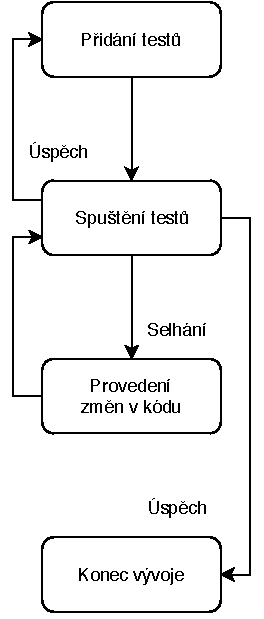
\includegraphics[width=.4\textwidth]{diagrams/TDD}
	\caption{Testy řízený vývoj softwaru}\label{fig:tdd}
\end{figure}

\section{Unit testování}

Unit testy slouží k ověřování funkcionality celků, v tomto případě tříd a jejich metod. V projektu je využíván framework MSTest V2~\cite{mstest}. Testy jsou umístěny v~jmenném prostoru  \mintinline{csharp}|ThermostatControler.Tests|.

Testy se snaží co nejvěrněji simulovat vstupy, které třída může dostat. Toho je docíleno dvěma způsoby:

\begin{enumerate}
	\item Generováním náhodných dat.
	\item Vytvářením dat pokrývajících co největší množství možných vstupů.
\end{enumerate}

Ke generování náhodných dat je využita třída \mintinline{csharp}|Generator|, umožňující vytvářet náhodné rozvrhy vytápění. Toto velice zjednodušuje testování, jelikož je možné generovat objekty obsahující desítky záznamů, které by bylo pracné vytvářet ručně. 

\begin{minted}{csharp}
List<Schedule> l = new List<Schedule>{Generator.GetSchedule(10)};
\end{minted}

Tímto voláním se vytvoří rozvrh vytápění, obsahující deset záznamů pro každý den. Nevýhodou tohoto přístupu je, že test nemusí pokaždé selhat a~nejsou přímo vidět data, na kterých selhal.

Nejlepším způsobem testování je projití všech možných vstupů, toho však v~pra\-xi často nelze dosáhnout. U ukládání uživatelských jmen je nemožné projít každou možnou kombinaci znaků, kterou uživatel může zadat -- délka jména není omezena. Proto jsou opět generována náhodná jména a hesla o~maximální délce 255 bytů.

\begin{minted}{csharp}
name = new byte[random.Next(255)];
pass = new byte[random.Next(255)];
random.NextBytes(name);
random.NextBytes(pass);
users.Add(new User(Convert.ToBase64String(name),
                   Convert.ToBase64String(pass)));
\end{minted}

Další test prochází všechny tisknutelné znaky z ASCII tabulky \cite{ascii}. Ty jsou spojeny do jednoho řetězce, představujícího uživatelské jméno. Tímto způsobem se sice nevytvoří všechna možná jména, ale otestuje se, zda se všechny znaky ukládají a načítají korektně.

Tyto ukázky jsou převzaté z testů pro třídu \mintinline{csharp}|Data|, avšak podobné techniky jsou využity i pro ostatní třídy.

\section{Manuální testování}

Manuální testování vyžaduje, aby testy provedl člověk – toto je velice časově náročné, člověk může udělat chybu a testy nejsou snadno opakovatelné. Z~těchto důvodů práce využívá co nejvíce automatizovaných testů. Některé testy se ovšem těžko automatizují a manuální testování v těchto případech zabere méně času než tvorba automatických testů. Manuální testování je v~práci využito k~testování funkcionality, která se nemění – stačí ji otestovat pouze jednou (například že nelze vytvořit dva uživatele se stejným jménem) – nebo má přesně zadané parametry, které lze všechny jednoduše otestovat.

Při testování třídy \mintinline{csharp}|WifiClient|, zajišťující komunikaci s~právě jednou topnou hlavicí, bylo nutné otestovat, zdali se podařilo navázat spojení a~jestli komunikace probíhá v pořádku. Tento proces popisuje obrázek~\ref{fig:manualTest}.

\begin{figure}\centering
	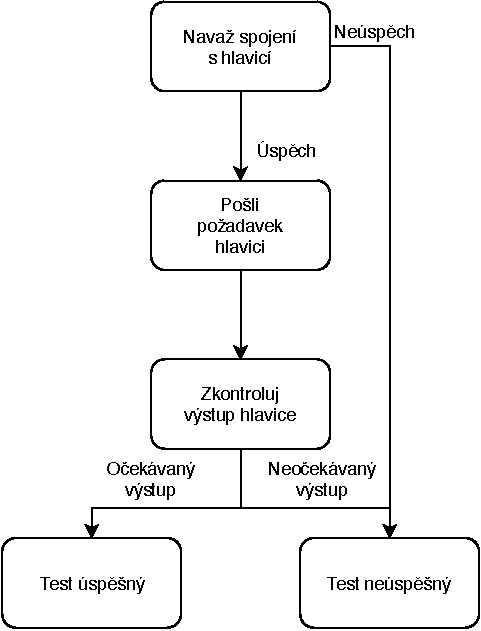
\includegraphics[width=.7\textwidth]{diagrams/ManualTest}
	\caption{Průběh manuálního testování}\label{fig:manualTest}
\end{figure}

Tester vždy musí zjistit IP adresu topné hlavice, kterou předá konstruktoru třídy \mintinline{csharp}|WifiClient|. Tuto funkcionalitu sice zajišťuje třída \mintinline{csharp}|WifiDevices|, ale testy by měly být závislé na co nejmenším počtu ostatních tříd. Třída \mintinline{csharp}|WifiClient| ke své funkci nutně nepotřebuje třídu \mintinline{csharp}|WifiDevices| a~proto v~testech není použita. Třída \mintinline{csharp}|WifiDevices| potřebuje metody z třídy \mintinline{csharp}|WifiClient|, pro provedení některých testů. Třída \mintinline{csharp}|WifiClient| je však v~tuto dobu již otestována a~je považována za funkční. Snížením závislostí, které na sebe třídy při testování mají, se zjednoduší případné hledání chyb.

Třída \mintinline{csharp}|WifiDevices| obsahuje metody pro vyhledávání zařízení (notebook, mobilní telefon\dots{}) a topných hlavic připojených k Wi-Fi síti. Tester tedy musí zjistit IP adresy zařízení připojených k síti a ty porovnat s výstupem testované metody. Tyto testy opět není možné jednoduše automatizovat, protože počty a IP adresy zařízení se můžou v čase měnit.


\section{Uživatelské testování}

Když aplikace obsahovala všechny funkce, bylo přistoupeno k uživatelskému testování. Pro testování byl vytvořen scénář, který měl tester projít a následně vyplnit dotazník. Po dobu testování byli testeři sledováni a v případě nutnosti proběhla diskuze nad problémy co objevili a jak by je vyřešili. Po každém testování byl projit dotazník, kde testeři popsali problémovou funkcionalitu – popřípadě návrhy na zlepšení aplikace. Tyto poznatky byly vyhodnoceny a~aplikace upravena. Další tester používal již upravenou verzi aplikace.

\subsection{Simulovaný kontrolér}

Pro nedostatek topných hlavic dostupných pro testování, byla vytvořena třída \mintinline{csharp}|SimulatedController|, poskytující falešné topné hlavice. Třída nahrazuje veškerou komunikaci s topnými hlavicemi novými metodami. Ostatní metody dědí ze třídy \mintinline{csharp}|Controller|. \mintinline{csharp}|SimulatedController| přidává topné hlavice, dokud jich v systému není osm.

\mintinline{csharp}|SimulatedController| v aktuální verzi aplikace nahrazuje \mintinline{csharp}|Controller| ve třídě \mintinline{csharp}|Presenter|, kde dovoluje zobrazovat více topných hlavic, se kterými mohli testeři interagovat. Zároveň bylo upraveno rozložení elementů, které vypisovaly topné hlavice na obrazovku.

\subsection{Testovací scénář}

Úkolem testovacího scénáře bylo projít všechny důležité funkcionality aplikace.

\begin{enumerate}
\item Přihlášení do aplikace a změna hesla.
\item Vytvoření rozvrhu vytápění.
\item Načtení a úprava rozvrhu vytápění.
\item Vytvoření profilu vytápění.
\item Nastavení režimu dovolené.
\item Úprava profilu vytápění.
\end{enumerate}

\subsection{Výsledky testování}

Testeři byli dotazováni na celkové hodnocení aplikace, zde byla vidět odlišnost mezi testery z technických a netechnických oborů. Testeři z netechnických oborů měli více výtek, co se týče vzhledu aplikace a rozložení jednotlivých elementů na obrazovce. Naopak testeři z technických oborů chtěli, aby aplikace co nejvíce zjednodušovala práci (výběr více položek najednou atd.), druhé skupině naopak nevadilo zadávat údaje ručně. Testeři z technických oborů upřednostňovali rychlost práce a~množství funkcí na úkor vzhledu aplikace. 

Na základě těchto výsledků bylo upraveno rozhraní aplikace, aby umožnilo rychlou změnu nebo vybrání více údajů najednou:

\begin{itemize}
\item Tlačítko pro zvolení všech dnů při tvorbě rozvrhu.
\item Volba jednoho rozvrhu pro všechny topné hlavice v profilu vytápění.
\item Přidávání dnů při opakovaném výběru rozvrhu vytápění pro editaci.
\end{itemize}

Aplikace byla upravena i po vizuální stránce:

\begin{itemize}
\item Změna rozmístění elementů na obrazovce.
\item Přidání chybějících popisků.
\item Upravení textů popisků pro upřesnění významu.
\end{itemize}

Všichni dotázání by aplikaci používali, zejména kvůli svým vlastním negativním zkušenostem s ovládáním termostatů a pro možnost kontroly teploty v jednotlivých místnostech.

\begin{conclusion}
Cílem této práce bylo navrhnout a implementovat aplikaci a topnou hlavici, které budou vzájemně komunikovat. Hlavním cílem aplikace bylo poskytnutí rozhraní pro usnadnění ovládání vytápění v domácnosti a nahradit dedikovaný hardware, který se k ovládání využívá.

Těchto cílů bylo dosaženo, i když „usnadnění ovládání“ je velice subjektivní pojem. Proto byla aplikace testována uživateli různých zájmových skupin. Z~výsledku testování vyplývá, že uživatelé byli schopni zvládnout zadané úkoly, aniž by byli s aplikací předem seznámeni, neměli problém osvojit si její ovládání a~funkcionality.

Aplikace obsahuje funkce pro rychlou změnu požadované teploty -- tvorbou rozvrhů vytápění, které jsou přiřazeny topným hlavicím. Pro změnu nastavení všech topných hlavic najednou, uživatel vytvoří seznam topných hlavic a jejich vytápěcích rozvrhů, který uloží do vytápěcího profilu. Přepínáním mezi profily, je možné měnit teplotu v celé domácnosti dvěma kliknutími.

Režim dovolené, který umožňuje temperovat domácnost na určenou teplotu, byl rozšířen o možnost přiřazení profilu, podle kterého se má do stanoveného data vytápět. Tato změna umožňuje zvolit si pro každou topnou hlavici jinou teplotu.

Aplikace umožňuje tvorbu uživatelských účtů, mající omezená oprávnění.

Součástí práce je i implementace topné hlavice komunikující s aplikací. Topná hlavice podle svého nastavení a aktuální teploty vypočítá, na kolik procent má být otevřen ventil radiátoru.

Do budoucna by bylo dobré pořídit více topných hlavic a otestovat spolehlivost aplikace s více připojenými hlavicemi. Další vylepšení by se mohla provádět na straně topné hlavice, která by mohla detekovat otevřená okna a~přizpůsobit se místnosti, ve které je radiátor umístěn. 

	
\end{conclusion}

\bibliographystyle{csn690}
\bibliography{mybibliographyfile}

\appendix

\chapter{Seznam použitých zkratek}
% \printglossaries
\begin{description}
	\item[DHCP] Dynamic Host Configuration Protocol
	\item[DNS] Domain Name System
	\item[EEPROM] Electrically Erasable Programmable Read-Only Memory
	\item[IPv4] Internet Protocol version 4
	\item[NTP] Network Time Protocol
	\item[SHA1] Secure Hash Algorithm 1
	\item[SSID] Service Set Identifier
	\item[TCP] Transmission Control Protocol
	\item[UDP] User Datagram Protocol
	\item[XML] Extensible markup language
\end{description}

\chapter{Obsah přiložené karty}

%Vhodným způsobem vizualizujte obsah přiloženého média. Lze použít balíček \verb|dirtree| a vytvořit např. následující výstup (adresáře src a text s~příslušným obsahem jsou \emph{povinné}):

\begin{figure}
	\dirtree{%
		.1 readme.txt\DTcomment{stručný popis obsahu karty}.
		.1 exe\DTcomment{adresář se spustitelnou formou implementace}.
		.1 src.
		.2 impl.
		.3 heater\DTcomment{zdrojové kódy topné hlavice}.
		.3 thermostatController\DTcomment{zdrojové kódy aplikace}.
		.2 thesis\DTcomment{zdrojová forma práce ve formátu \LaTeX{}}.
		.1 text\DTcomment{text práce}.
		.2 thesis.pdf\DTcomment{text práce ve formátu PDF}.
	}
\end{figure}


\end{document}
